\documentclass{article}
\usepackage[utf8]{inputenc} % allow utf-8 input
\usepackage{amsfonts}       % blackboard math symbols
\usepackage{color}
\usepackage{amsmath}
\usepackage{graphicx}


\title{AM205: Introduction to Compiled Languages: exercise in C++ and data visualization}
\author{Yuexia Luna Lin, Baptiste Lemaire, Nick Derr}

\begin{document}
\maketitle

\section*{Newton method and Newton fractal}
As we will cover soon in the course, Newton's method, also known as the Newton-Raphson method, is widely used in finding the roots of a function.
Assume we have an initial guess, $x_0$, and it's close to a root, then function $f(x)$ can be approximated by its first order Taylor expansion,

$$
	f(x_0 + \Delta x) = f(x_0) + f'(x_0) \Delta x
$$

If this approximation is good, if we set $f(x_0 + \Delta x) = 0$, we can solve for the location of the root, 
$$
   \Delta x = -\frac{f(x_0)}{f'(x_0)}; ~~x_r = x_0 + \Delta x
$$
However, in actuality, the approximation may not be good enough, but the above reasoning
gives us an iteration rule, or a recurrence relation,
$$
x_1 = x_0 + \Delta x = x_0 - \frac{f(x_0)}{f'(x_0)}
$$
or more in general,
$$
x_{n+1} = x_n  -\frac{f(x_n)}{f'(x_n)}
$$

There are some caveats to this rule, especially in tricky cases where the assumptions of (1) initial guess being close to a root (2) the function having a continuous, non-zero first derivative, are violated.
Usually, if a division by zero happens, we terminate the iterations, change the initial guess and try again. Sometimes, the algorithm can get stuck in a cycle.\footnote{Just try apply Newton's method to $f(x) = x^3 - 2x + 2$, with initial guess $x_1 = 1$.}
In practice, we set a threshold of error tolerance, $tol$, such as the algorithm is
terminated if 
\begin{equation}
| x_{n+1} - x_{n} | < tol
\label{eq:thres}
\end{equation}
 is reached. Besides that, we also impose a limit on the number of maximum iterations the algorithm can take,
so that we can terminate the algorithm gracefully when it has failed to converge. 

A good initial guess can help Newton's method converge very rapidly, a bad one would make it stuck in a cycle forever or diverge.
But there isn't a steadfast rule to discern which initial guess would converge to which root. This is where the plot thickens.

We know that polynomials can have complex roots. 
Newton's method can be adapted to find the roots of polynomial $p(z)$ of complex argument $z$ in the complex plane.
The regions that converge to a particular root is called the basins of attraction for that root. 
One might expect there to be a clean cut boundary dividing these regions, because we
may think that a point closer to a root would converge to that root. Not so!
The boundaries between basins of attractions, in polynomials of degree $>2$, are \textbf{fractal}.

If we color the basin of attraction for a root in the complex plane by the same color, we will see some amazing patterns.
Figure~\ref{fig:nfrac} shows such an example from \textit{Wikipedia} for polynomial $p(z)=z^3-1$, whose roots are $1, -\frac12 \pm \frac{\sqrt{3}}{2} i$. 
The basins of attraction for $1$ are colored shades of yellow, those for $-\frac12 + \frac{\sqrt{3}}{2}$ are colored shades of magenta, and those for  $-\frac12 - \frac{\sqrt{3}}{2}$ are colored shade of cyan. 
We indeed see that in the boundaries between the large basins of attraction have fractal structure\footnote{Visit  \color{blue} {http://usefuljs.net/fractals/docs/newtonian\textunderscore fractals.html }\color{black} for a fun read, and an online fractal generator!}.
Patterns like these are called the Newton fractals.
 
 \section*{Workshop report}
 1. Your first exercise is to reproduce Figure~\ref{fig:nfrac} using the complex version of Newton's method\footnote{See   \color{blue} https://en.wikipedia.org/wiki/Newton\textunderscore fractal \color{black} for details.},
 \begin{equation}
 z_{n+1} = z_n - \frac{p(z_n)}{p'(z_n)}
 \label{eq:cnewton}
 \end{equation}
 for polynomial $p(z)=z^3-1$. The first derivative\footnote{This function is analytic in the context of complex analysis. Its derivative can be written as $p(z) = \frac{dp(z)}{dz}$.}, $p'(z) = 3z^2$.  To compute these arithmetics in the complex plane, use the \texttt{complex<double>} type in the STL library. (You will find example \texttt{complex\textunderscore num.cc} in the GitHub repo\footnote{\color{blue}https://github.com/ylunalin/am205\textunderscore compiled\textunderscore lang.git\color{black}}  on how to use this data type.)
 
Discretize a part of the complex plane, $[ -L, L]\times [-iL, iL ]$ , with $N\times N$ grid points; the grid spacing is $\Delta h = \frac{2L}{N-1}$.
Define $z_{00} = -L - iL$, the complex number of at grid point indexed with $(m,n)$ is $z_{mn} = z_{00} + m \Delta h + i n \Delta h$, for $m, n \in [0, N-1]$. 

Perform iterations defined by Eqn.~\ref{eq:cnewton} using each grid point as an initial guess, and keep track which root this guess has converges to, e.g. you can use 0 to indicate failure to converge, 1, 2, and 3 as root markers. 
Make sure to set two termination conditions, one checking that the iteration has converged (Eqn.\ref{eq:thres}) and the other limit the maximum number of iteration allowed. 

To make sure the resolution of your image is good, you should use $dh<0.005$.
Use your preferred data plotting software to visualize the end results. For example, in python, you can use \texttt{matplotlib.pyplot.imshow}. A command line plotting tool called \texttt{Gnuplot} is also very useful.
You can beautify the figure by using some nice palettes. (You will find \texttt{gnuplot\textunderscore example.gp} on the GitHub repo with codes to plot a sample dataset with a nice purple palette in \texttt{Gnuplot}.)
\\

2. Now that you have the code working to create a Newton fractal for $p(z) = z^3-1$, choose another polynomial, and see what Newton fractal you can create!
\\

3. Submit an one-page write-up along with your \textbf{code}. The write-up should 
\begin{itemize}
 \item Include a plot of your reproduction of Figure \ref{fig:nfrac} in a palette different from the original. Report your parameters, $L$ and $N$, and the total time of computation.
 \item Present the polynomial of degree $>2$ of your choosing. Include a plot of your very own Newton fractal. Report your parameters, $L$ and $N$, and the total time of computation.
\end{itemize}
Good luck and have fun!
 
\begin{figure}[t]
\centering
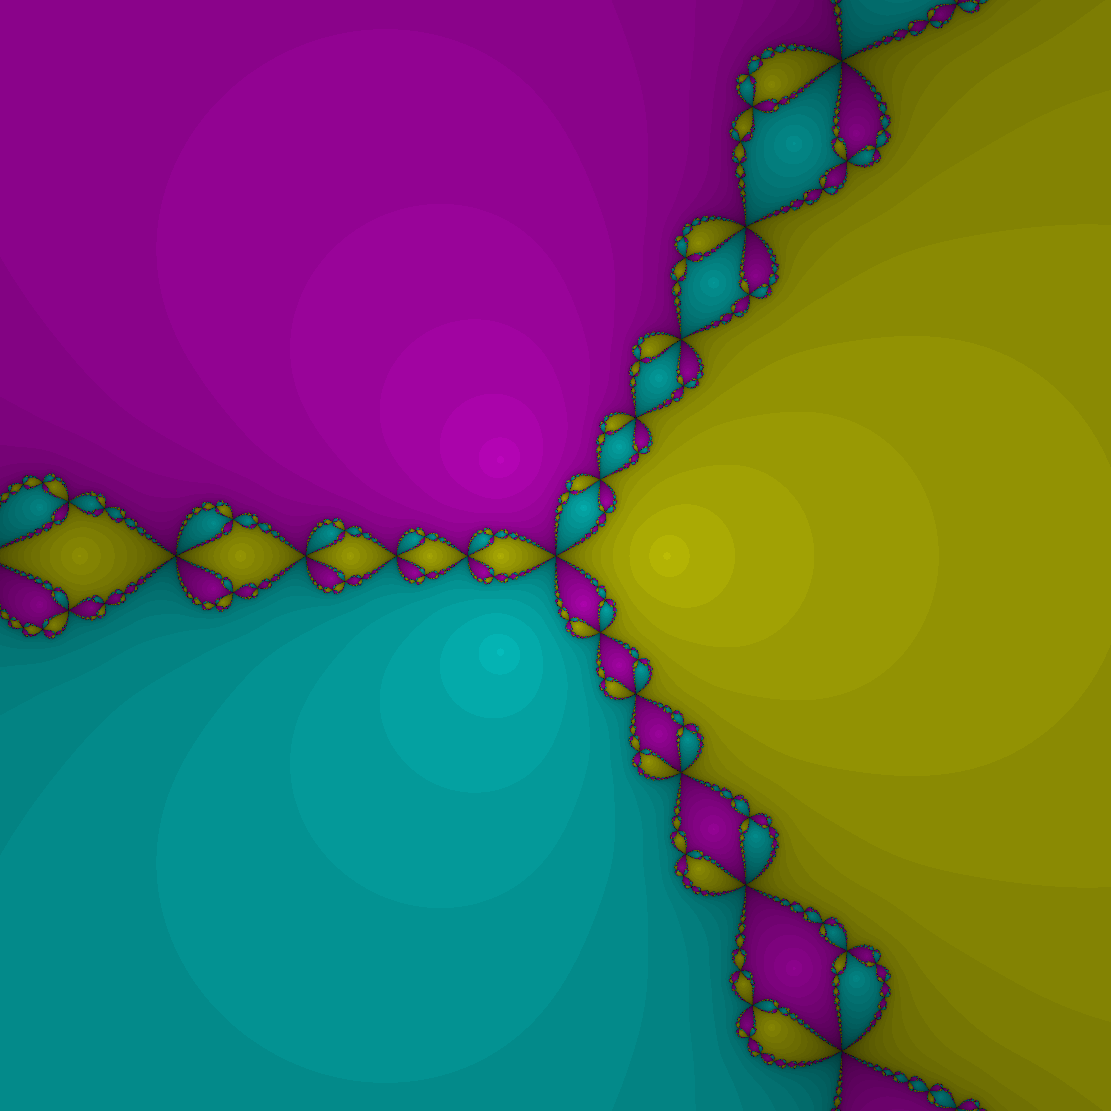
\includegraphics[width = \linewidth]{Newtroot_1_0_0_m1.png}
\caption{Newton fractal for complex polynomial $p(z) = z^3 - 1$. Credit: Wikipedia user LutzL.}
\label{fig:nfrac}
\end{figure}

\end{document}
